\section{Cel dokumentu}\label{cel-dokumentu}

Niniejszy dokument opisuje schemat postępowania w projekcie, poczynając
od zebrania danych aż do ich analizy.

\section{Schemat postępowania:}\label{schemat-postepowania}

Poniższy schemat przedstawia zarys postępowania w projekcie, wstępnie
określa jego fazy, które są dokładniej scharakteryzowane w dalszej
części dokumentu.

\centerline{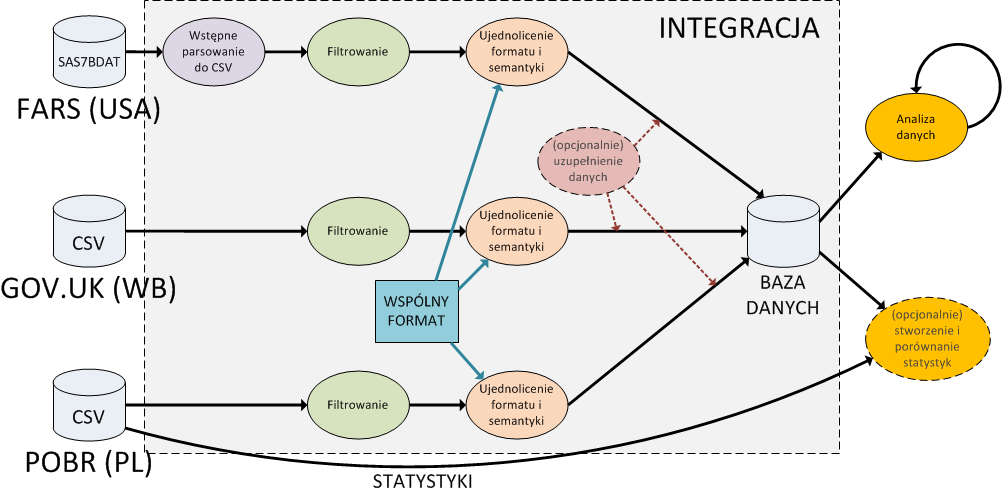
\includegraphics[width=0.9\textwidth]{images/schemat_integracji.png}}

\section{Pobranie danych}\label{pobranie-danych}

W wyniku przeprowadzonej analizy źródeł danych, której rezultaty zostały
przedstawione w dokumencie \href{Analiza-źródeł-danych}{Analiza żródeł
danych}, wytypowane zostały źródła danych, które zostaną wykorzystane w
projekcie. Pierwszą fazą realizacji projektu jest uzyskanie dostępu do
danych, oraz pobranie ich ze źródeł. Wybrane dane pochodzą z trzech
krajów.

\begin{itemize}
\itemsep-14pt\parskip0pt\parsep0pt
\item
  Polska - dane Polskiego Obserwatorium Ruchu Drogowego\\
\item
  Wielka Brytania - dane z witryny gov.pl\\
\item
  Stany Zjednoczone - dane z systemu FARS - Fatality Analysis Reporting
  System
\end{itemize}

W przypadku niektórych źródeł dane są dostępne do pobrania bezpośrednio
ze strony lub serwera ftp, bez ograniczeń dostępu, jednak w przypadku
danych z POBR konieczne jest uzyskanie dodatkowej autoryzacji w celu
skorzystania z pełnych danych, więc dla tego źródła danych konieczny
jest właśnie ten dodatkowy krok.

\section{Filtrowanie danych}\label{filtrowanie-danych}

Dane ze źródeł muszą następnie zostać odfiltrowane. Jest to umotywowane
zarówno dużą ilością danych jak i procesem preintegracji danych.
Dodatkowym ograniczeniem są podjęte przez nas decyzje projektowe
zawężające celowo zakres danych.

Filtrowanie danych będzie przebiegać na trzech płaszczyznach:

\begin{itemize}
\itemsep-14pt\parskip0pt\parsep0pt
\item
  stopień powagi wypadku: podjętą przez nas decyzją projektową chcemy
  się ograniczyć do wypadków śmiertelnych, będziemy więc gromadzić
  jedynie dane o takich wypadkach, odrzucając wypadki lekkie i poważne,
  ale bez skutków śmiertelnych\\
\item
  czas (wybrane roczniki) w celach interacyjnych: chcemy ograniczyć się
  do roczników, z których dane są dostępnych we wszystkich źródłach w
  celu lepszych możliwości porównania\\
\item
  czas (wybrane roczniki) w celach zapewnienia pełności danych: chcemy
  odrzucić dane z lat, dla których mamy ich zbyt mało - zakres atrybutów
  był zbyt wąski lub większość informacji jest niedostępna. Może być to
  szczególnie widoczne w danych starszych.
\end{itemize}

\section{Uwspólnienie formatu i semantyki danych}\label{uwspolnienie-formatu-i-semantyki-danych}

W celu analizy danych zróżnych źródeł konieczne jest ustalenie wspólnego
formatu danych. obejmuje on zarówno kwestie wspólnego formatu (np.
wspólny format daty), ale również uwspólnienie semantyki - przykładem
może byc opis warunków pogodowych: różne bazy przedstawiają te dane w
różny sposób, różną gamą możliwych wartości atrybutu, konieczne jest
ustalenie wspólnej listy wartości atrybutów, na którą następnie będzie
można zmapować atrybuty z poszczególnych źródeł.

Ważnym zadaniem tego etapu jest selekcja atrybutów, które będą dla nas
istotne w przeprowadzanych analizach, w szczególności selekcja atrybutów
pozwalających wnioskować o przyczynach wypadków - kryteria analizy.
Kryteria te możemy podzielić na następujące ogólne kategorie:

\begin{itemize}
\itemsep-14pt\parskip0pt\parsep0pt
\item
  data\\
\item
  miejsce\\
\item
  warunki pogodowe\\
\item
  warunki środowiskowe\\
\item
  dane o uczestnikach (np. młodzi / pijani kierowcy)\\
\item
  dane o pojazdach (np. rocznik, systemy bezp.)
\end{itemize}

Dokładny opis szczegółowych kryteriów analizy można znaleźć w dokumencie
\href{Kryteria-analizy}{Kryteria analizy}.

\section{Integracja}\label{integracja}

Integracja danych polegać będzie na sprowadzeniu danych do określonego
wcześniej wspólnego formatu. W tym celu konieczne będzie sparsowanie
danych przy pomocy skryptów w pythonie a następnie przetłumaczenie i
zmianę formatu na wspólny.

W miarę potrzeby i możliwości będziemy również na tym etapie uzupełniać
dane z dodatkowych źródeł - np. w razie braku danych o pogodzie dla
dużej ilości wypadków, można z innych źródeł pobrać informacje o
pogodzie w danym miejscu i czasie.

Tak przetłumaczone i uzupełnione dane zostaną zapisane do relacyjnej
bazy danych PostgreSQL, zgodnie z opracowanym schematem bazy danych,
który jest dokładnie opisany w dokumencie
\href{Projekt-bazy-danych}{Projekt bazy danych}.

\section{Analiza danych}\label{analiza-danych}

Kolejnym, kluczowym krokiem procesu jest analiza danych. Dane
zgromadzone w bazie będziemy analizować na kilka sposobów.

Pierwszym z nich jest analiza statystyczna. Przy pomocy narzędzi do
wizualizacji oraz narzędzi analizy statystycznej języka R czy platformy
Weka będziemy analizować statystyczne własności danych takie jak
korelacje czy procentowe udziały atrybutów. Głównymi atrybutami branymi
pod uwagę w tej analizie będą atrybuty wskazane w dokumencie
\href{Kryteria-analizy}{Kryteria analizy}. W ramach analizy wizualnej
będziemy rozważać wykresy generowane z danych a także nanosić dane na
mapy w celu dokonania przestrzennej analizy danych.

Z bardziej zaawansowanych metod, chcemy spróbować poddać dane
klasteryzacji w celu wskazania podobnych wypadków i podjęcia próby
wskazania dla nich wspólnych cech. Dodatkową formą analizy danych będzie
wyszukiwanie wzorców częstych - pozwoli ono wskazać często
współwystępujące okoliczności wypadków i wysnuć wnioski co do ich wpływu
na występowanie wypadków.

\section{Opcjonalne kierunki analizy}\label{opcjonalne-kierunki-analizy}

Jeżeli po wykonaniu wymienionych już analiz zostanie nam nieco czasu,
możemy podjąć się zrealizowania w projekcie opcjonalnych kierunków
analizy. Będą one polegać na stworzeniu zbiorczych statystyk z danych
przechowywanych w bazie i porównanie ich ze zbiorczymi danymi z
regionów, dla których nie mamy dostępu do szczegółowych danych z
wypadków. Chodzi tu szczególnie o dane z Polski, dla których nie mamy
pewności, że uda nam się otrzymać do nich dostęp.

\section{Używane technologie}\label{uzywane-technologie}

W projekcie będą wykorzystywane następujące narzędzia i technologie:

\begin{itemize}
\item
  python - \url{https://www.python.org/}

  \begin{itemize}
  \itemsep-14pt\parskip0pt\parsep0pt
  \item
    skrypty filtrujące / parsujące / konwertujące\\
  \item
    parser sas7bdat - \url{http://github.com/openfisca/sas7bdat}\\
  \end{itemize}
\item
  PostgreSQL - \url{http://www.postgresql.org/}

  \begin{itemize}
  \itemsep-14pt\parskip0pt\parsep0pt
  \item
    relacyjna baza danych do persystencji\\
  \end{itemize}
\item
  Narzędzia do analizy danych:

  \begin{itemize}
  \itemsep-14pt\parskip0pt\parsep0pt
  \item
    MS Excel\\
  \item
    R - \url{http://www.r-project.org/}\\
  \item
    Weka - \url{http://www.cs.waikato.ac.nz/ml/weka/}\\
  \end{itemize}
\item
  Narzędzia do wizualizacji danych

  \begin{itemize}
  \itemsep-14pt\parskip0pt\parsep0pt
  \item
    Polymaps - \url{http://polymaps.org/}\\
  \item
    Google Charts - \url{https://developers.google.com/chart/}\\
  \item
    OpenLayers - \url{http://openlayers.org}
  \end{itemize}
\end{itemize}

\section{Referencje}\label{referencje}

\begin{enumerate}
\itemsep-14pt\parskip0pt\parsep0pt
\item
  POBR - \url{http://www.obserwatoriumbrd.pl/}\\
\item
  FARS - \url{http://www.nhtsa.gov/FARS},
  \url{ftp://ftp.nhtsa.dot.gov/FARS/}\\
\item
  Dane z Wielkiej Brytanii -
  \url{http://data.gov.uk/dataset/road-accidents-safety-data}
\end{enumerate}
